\section{Expérience D1} 
  \subsection{Objectif}
    En utilisant la seconde architecture de \cite{Cleeremans_2007}, 
    comprendre de quelles manières un réseau de neurone connexionniste peut, à partir de ses propres paris
    sur son résultat, améliorer son comportement.
  
  
     
  \subsection{Architecture}
    \paragraph{Description}
      Un premier réseau de perceptron multicouche apprend à discrétiser des chiffres représentés
      par 256 (16x16) neurones d'entrées. Il est composé d'une couche cachée de 100 neurones.
      
      Un second réseau de perceptron multicouche apprend à parier sur la qualité de la réponse
      du premier réseau à partir de sa couche cachée.
      
      L'apprentissage du second réseau, n'affecte pas les poids entre la couche d'entrée et la 
      couche cachée du premier réseau.
      
      Lorsque le second réseau parie haut, la réponse du premier réseau est gardée, à l'inverse,
      lorsqu'il parie bas, c'est le second neurone le plus élevé du premier réseau qui sera 
      la réponse.


    \paragraph{Schéma}
      \begin{center}
	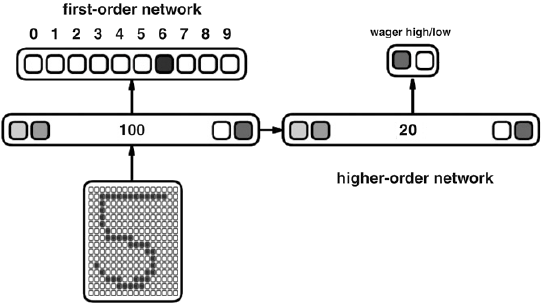
\includegraphics[width=250px]{data/expD1/schema.png}
      \end{center}
      
    \paragraph{Paramètres}
      \begin{center}
	\begin{tabular}{lr}
	  \begin{minipage}{230px}
	    \begin{itemize}
	      \item momentum : 0.5 sur le premier réseau
	      \item momentum : 0. sur le second réseau
	      \item taux d'apprentissage : 0.15 sur les 2 réseaux
	      \item \textbf{1600 formes} de chiffres différents présentées (shuffle) \cite{Handwritten_256}
	      \item apprentissage 50 (formes) x 300 (époques)
	      \item utilisation de biais
	      
	    \end{itemize}
	  \end{minipage}
	  &
	  \begin{minipage}{230px}
	    \begin{itemize}
	      \item poids initialisés sur [-1 ; 1] pour le premier réseau
	      \item poids initialisés sur [-0.25 ; 0.25] pour le second réseau
	      \item taux d'apprentissage constant
	      \item entrées valent 0 ou 1
	      \item sigmoïde à température 1
	    \end{itemize}
	  \end{minipage}
	\end{tabular}
      \end{center}

  
  \newpage
  \subsection{Résultats}
    \paragraph{Principaux}
      Analyse des performances
      \begin{center}
	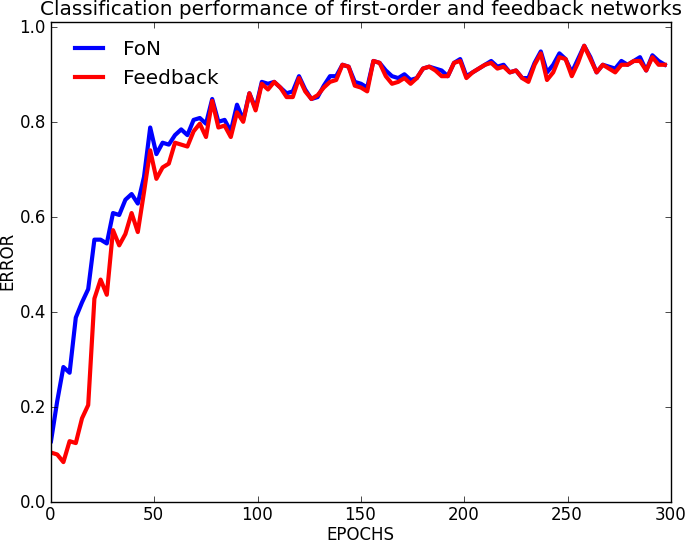
\includegraphics[width=250px]{data/expD1/perff.png}
      \end{center}
      \subparagraph{Notes}
	\begin{itemize}
	  \item la performance de classification représente le taux de bonnes réponses (winner-take-all) pour les 50 formes présentées sur une époque
	\end{itemize}
      \subparagraph{Conclusion}
	\begin{itemize}
	  \item l'architecture n'arrive pas à obtenir une augmentation de performance, ce qui veut dire que la bonne réponse ne se trouve pas dans
	  le second neurone le plus élevé (lorsque la réponse n'est pas dans le premier).
	\end{itemize}
    \paragraph{Secondaires}
      Analyse des performances sous-jacentes
      \begin{center}
	\begin{tabular}{lr}
	  \hspace*{-1cm}
	  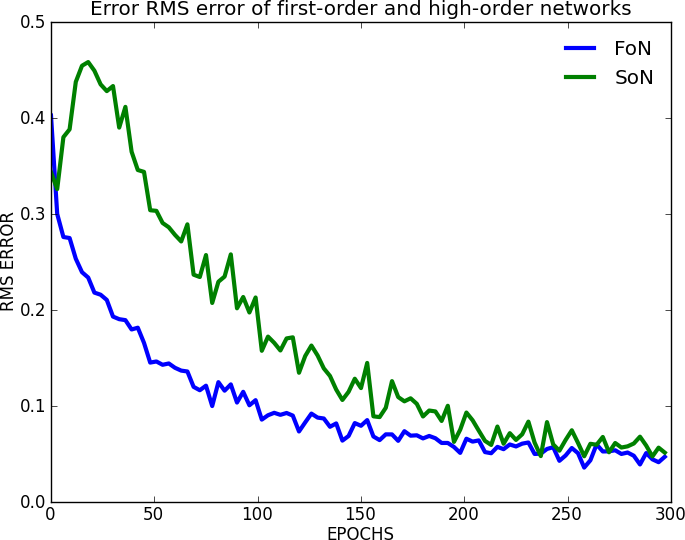
\includegraphics[width=250px]{data/expD1/rms.png}
	  &
	  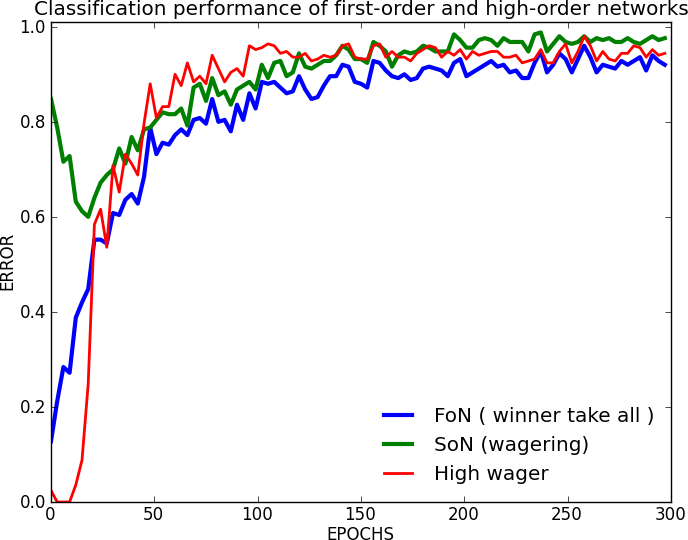
\includegraphics[width=250px]{data/expD1/perf.png} 
	\end{tabular}
      \end{center} 
      \subparagraph{Notes}
	\begin{itemize}
	  \item la courbe rouge représentent le taux de paris hauts du second réseau
	  \item la performance de classification représente le taux de bonnes réponses (winner-take-all) pour les 50 formes présentées sur une époque
	  \item formule utilisée pour RMS (cf. Formules~\nameref{rms})
	\end{itemize}
      \subparagraph{Conclusion}
	Les performances du second réseau sont respectables ceci prouve bien l'hypothèse précédente.


  \subsection{Conclusion}
  Lorsque la réponse n'est pas dans le neurone le plus élevé, elle ne se trouve pas non plus toujours 
  dans le second neurone le plus élevé.
  
  
  Cette idée nous ouvre le chemin vers l'\nameref{expD2} qui tentera d'enregistrer la profondeur de la bonne réponse.
  \newpage 
  \subsection{Formules}
    \paragraph{RMS} \label{rms}
  Pour une époque $e$ :
  \begin{center}
    \begin{large}
    $ rms_{e} = \sqrt{ \frac{1}{n} \sum \limits_{i=1}^{n} 
    ( o_{i,e} - d_{i} )^2 } $
    \end{large}
  $ with \left\lbrace \begin{array}{lll} n : number\ of\ neurons\ on\ the\ output\ 
  layer\\o_{i,e} : value\ obtained\ for\ the\ i^{th}\ neuron\ at\ the\ e^{th}\ epoch\\d_{i} : 
  value\ desired \ for\ the\ i^{th}\ neuron\end{array} \right.$
  \end{center}
    
    \paragraph{Descente de gradient} \cite{Touzet_1992} \\
  Construction de l'erreur : 
    \begin{center}
      $y_{i} = f'(a_i) \times ( d_i - x_i ) \ si\ i\ neurone\ de\ sortie $ \\
      $y_{i} = f'(a_i) \times \sum \limits_{k} ( w_{ki} \times y_k )\ si\ i\ neurone\ cache $
    \end{center}
  Mise à jour des poids :
    \begin{center}
      $w_{ij}(t+1) = w_{ij}(t) + learning\_rate \times y_{i} \times x_j + momentum \times 
      (w_{ij}(t) - w_{ij}(t-1) )$
    \end{center}
  Variables : 
    \begin{center}
      $\left\lbrace \begin{array}{lll} 
	f : fonction\ sigmoide \\
	x_i : valeur\ du\ neurone\ i\\
	d_i : valeur\ desire pour\ le\ neurone\ i\\
	a_i : somme\ pondere\ des\ poids\ du\ neurone\ i
      \end{array} \right.$
    \end{center}
    
\bibliographystyle{../pre-rapport/apalike}
\bibliography{../pre-rapport/biblio}
